\documentclass[manuscript,review,anonymous]{acmart}

\setcopyright{none}
\citestyle{acmauthoryear}

\acmConference[Collective Intelligence]{ACM Collective Intelligence}{2026}{TBD}
\acmYear{2026}
\acmBooktitle{Proceedings of ACM Collective Intelligence}

\begin{document}

\title[Legislative Design Space]{Searching Legislative Design Space for Compromise and Productivity}
\subtitle{A Computational Framework for Comparing Congress-Style Institutional Designs}

\author{Anonymous Author(s)}
\affiliation{%
  \institution{Anonymous Institution}
  \country{Anonymous Country}
}
\renewcommand{\shortauthors}{Anonymous Author(s)}

\begin{abstract}
Legislatures need enough productivity to act, but productivity alone can also mean volatility, agenda capture, or weakly supported lawmaking. This paper presents a reproducible computational framework for searching legislative design space rather than defending any single reform. The simulator routes shared synthetic legislatures and bill streams through Congress-style institutional bundles that vary agenda access, voting thresholds, alternative selection, citizen review, lobbying safeguards, affected-group protection, package bargaining, and reversibility.

The contribution is methodological. The simulator separates productivity from compromise, public alignment, weak public-mandate passage, policy yield per submitted proposal, pre-floor blockage reliance, proposer advantage, concentrated harm, lobbying capture, administrative cost, and correction over time. One main comparison campaign generates the central scenario tables and scatter figures, while separate scripted diagnostics generate seed, ablation, manipulation-stress, chamber-structure, and empirical-bridge checks. The current experiment is breadth-first: default enactment remains one burden-shifting stress test, while the main comparison spans conventional, deliberative, anti-capture, agenda-scarcity, policy-tournament, harm-protection, and review-oriented families. The paper argues for mechanism search: legislative designs should be compared as portfolios of incentives and safeguards, not as isolated passage thresholds.
\end{abstract}

\begin{CCSXML}
<ccs2012>
<concept>
<concept_id>10003120.10003121.10003124.10010392</concept_id>
<concept_desc>Human-centered computing~Collaborative and social computing theory, concepts and paradigms</concept_desc>
<concept_significance>500</concept_significance>
</concept>
<concept>
<concept_id>10010147.10010257</concept_id>
<concept_desc>Computing methodologies~Modeling and simulation</concept_desc>
<concept_significance>500</concept_significance>
</concept>
<concept>
<concept_id>10010405.10010455.10010460</concept_id>
<concept_desc>Applied computing~Law</concept_desc>
<concept_significance>300</concept_significance>
</concept>
</ccs2012>
\end{CCSXML}

\ccsdesc[500]{Human-centered computing~Collaborative and social computing theory, concepts and paradigms}
\ccsdesc[500]{Computing methodologies~Modeling and simulation}
\ccsdesc[300]{Applied computing~Law}

\keywords{legislative institutions, institutional design, computational simulation, agenda control, compromise, collective decision-making, voting systems}

\maketitle

\section{Introduction}

The motivating question is not whether one unusual voting rule should replace Congress. It is whether systematic design search can help identify legislative structures that better combine productivity, compromise, and representative responsiveness. A legislature can be unified without being democratic; authoritarian systems can appear cohesive because disagreement is suppressed. A useful representative system should instead help actors with competing interests reach compromises connected to public support, public benefit, and the burdens imposed on affected groups.

Default enactment, where a proposal passes unless a blocking coalition stops it, is one design in the search space, not the object of the project. It is useful as a stress test because it reverses the usual burden of coalition formation. The broader object is the mechanism bundle around any final yes-or-no vote: who may propose, how agenda access is rationed, whether information is improved before voting, whether opponents have scarce challenge rights, whether bill content can move toward compromise, whether concentrated losers receive protection, and whether bad laws can be corrected later.

This paper therefore makes a modest claim. It does not validate a new constitution or forecast the U.S. Congress. It contributes an executable framework for comparing legislative mechanisms under common assumptions, with explicit metrics and reproducible artifacts. The simulations are comparative stress tests: they reveal when a rule produces output, when it produces compromise, and when those two diverge.

\section{Related Work}

The model draws on individual-level simulation, spatial voting, and institutional theory. Agent-based and computational political models are useful when heterogeneous actors interact under rules that create aggregate outcomes \citep{Epstein2006,GilbertTroitzsch2005,deMarchiPage2014}. Spatial voting motivates one-dimensional ideal points and status-quo-relative utility \citep{Downs1957}. Legislative bargaining and agenda-setter models motivate explicit proposer identity and proposer gain \citep{BaronFerejohn1989,RomerRosenthal1978}. Pivotal-politics and veto-player theories motivate comparing simple majority, supermajority, bicameral, and executive-veto systems \citep{Krehbiel1998,Tsebelis2002}. Committee and agenda-control theory motivates treating floor denial, referral, information, and amendment control as outcomes rather than missing observations \citep{CoxMcCubbins2005,GilliganKrehbiel1987,Krehbiel1991,Shepsle1979,ShepsleWeingast1987,WeingastMarshall1988}.

Several tested mechanisms come from adjacent literatures. Lobbying is modeled as access, effort, information, public pressure, and participation bias rather than only direct vote buying \citep{AustenSmith1993,AustenSmith1995,HallDeardorff2006,HallWayman1990,deFigueiredoRichter2014,GilensPage2014}. Citizen-panel variants draw on deliberative polling and mini-public practice \citep{Fishkin2009,OECD2020}. Agenda-credit variants echo quadratic-voting and storable-vote work on expressing intensity under scarcity \citep{Casella2005,LalleyWeyl2018}. Reversibility variants draw on temporary legislation and sunset review \citep{Gersen2007,Ranchordas2014}. Policy tournaments draw on Condorcet and agenda-manipulation problems \citep{McKelvey1976,Tideman1987}. Model documentation follows ODD and ODD+D conventions \citep{Grimm2010,Muller2013}.

Default-effect rules have real analogues, although usually in bounded domains: WTO dispute settlement, EU reverse-qualified-majority enforcement, tacit-acceptance procedures, and U.S. fast-track or disapproval structures all shift procedural burdens in limited ways \citep{WTO1994,EuropeanParliament2011,ChurchillUlfstein2000,CRA1996,CRSFastTrack2024}. These analogues suggest the same design lesson as the simulator: burden-shifting rules need guardrails around proposal access, objection, information, and correction.

\section{Simulator}

Each run creates a synthetic legislature, bill stream, status quo, and institutional process. Legislators have ideal points in \([-1,1]\), party labels, district preferences, and heterogeneous sensitivity to party pressure, constituency pressure, lobbying, reputation, and compromise. Bills have a proposer, policy position, public support, generated public benefit, lobby pressure, salience, private gain, issue domain, public-benefit uncertainty, affected-group support, and concentrated harm. Enacted bills update the status quo, so votes evaluate policy movement rather than isolated proposals.

The implementation separates voting rules from legislative processes. Voting rules interpret yes/no totals. Processes wrap a bill in stages such as proposal access, leadership control, committee assignment and gatekeeping, discharge-petition bypass, open floor calendars, citizen petitions, bicameralism, conference, veto, judicial review, coalition confidence, initiatives, lotteries, attention budgets, challenge vouchers, routing, norm erosion, sunset review, credits, bonds, lobbying, harm review, package bargaining, mediation, alternatives, amendment tournaments, citizen-panel review, objection, and law-registry review. Post-enactment review now tracks implementation delay, capacity, underfunding, nonenforcement, and renewal pressure as separate diagnostics. This modularity is central: the same threshold behaves differently when proposals are open, filtered, challenged, revised, reviewed, or made reversible.

The stylized U.S.-like conventional benchmark uses House majority passage, a Senate 60 percent threshold, presidential veto, two-thirds override, and an agenda-access gate. The gate prevents the benchmark from treating every introduced bill as a floor bill; it schedules bills using observable proxies: public support, salience, policy stability, sponsor-party fit, partisan queue conflict, capture risk, concentrated harm, and uncertainty. It does not observe generated public benefit directly. This makes the conventional baseline pass the current calibration screen without claiming it is a fitted model of Congress.

\section{Metrics and Campaign}

The simulator reports a dashboard rather than a single welfare score. Higher-is-better metrics include productivity, enacted support, generated welfare among enacted bills, policy yield, compromise, public alignment, legitimacy, citizen certification, district alignment, and anti-lobbying success. Lower-is-better metrics include gridlock, low-support or weak-mandate passage, popular failure, lobbying capture, public-preference distortion, minority harm, proposer gain, administrative cost, blockage reliance, low-support active-law share, and false-negative default passage. Floor consideration, access denial, committee rejection, challenge, amendment, compensation, reversal, attention spending, objection, and policy shift are diagnostic: high values can mean useful activity or institutional strain.

The metric types matter. Some metrics are structural outputs, such as productivity, enactment counts, floor load, review load, pre-floor blockage reliance, and administrative cost. Some are synthetic value proxies generated inside the model, such as public support, public benefit, legitimacy, weak public mandate, policy yield, and affected-group harm. Others are diagnostics, such as amendment overload, poison-pill risk, petition distortion, implementation failure, challenge, objection, and reversal rates. Chamber low-support passage is mainly a threshold-failure metric; under ordinary majority voting it is often mechanically low. Weak public-mandate passage is the cross-system public-support failure metric because it asks whether enacted bills had generated public support below 50 percent, regardless of the chamber vote rule.

For display, the paper reports a directional score only as a diagnostic reading aid. Representative quality now combines enacted-policy quality, policy yield per submitted proposal, and public-mandate legitimacy, so a system that looks good mainly by blocking most proposals is distinguished from one that actually produces public-value output. Risk control inverts chamber low-support passage, weak public-mandate passage, minority harm, lobbying capture, public-preference distortion, concentrated-harm passage, proposer gain, and policy shift. Administrative feasibility inverts estimated procedural load from attention spending, review, challenge, amendment, and alternative selection. The directional score averages productivity, representative quality, risk control, and administrative feasibility, but the analysis emphasizes Pareto tradeoffs because different value profiles favor different institutional designs.

All main results come from one reported comparison campaign. It combines broad assumptions, adversarial generator cases, weighted party-system cases, and a stylized rising-contention timeline in one CSV. Cases vary polarization, party loyalty, compromise culture, lobbying, constituency pressure, party count, proposal pressure, capture pressure, anti-lobbying reform demand, and six adversarial bill streams: high-benefit extreme reform, popular harmful bills, moderate capture, delayed-benefit reform, concentrated rights-like harm, and anti-lobbying backlash.

Scenario selection follows a fixed coverage rule: include conventional baselines, the stylized U.S.-like benchmark, readable representatives for implemented non-default design classes, and three default-enactment stress tests. The selection manifest records each row's role and rationale; \texttt{make family-screen} reports fixed-rule family champions. The main comparison now includes pre-floor mechanisms directly: proportional committees, discharge petitions, open floor calendars, citizen petitions, amendment tournaments, and anti-capture proposal access. Earlier default-pass sweeps remain side logs, not the organizing evidence base.

The chamber-structure supplement tests representation architecture, committee power, eligibility filters, and ex ante review. It is separate because it asks how those structures shift the same productivity/compromise tradeoff.

Calibration is a screening step, not a parameter fit. \texttt{make calibrate} compares conventional baselines with broad benchmark ranges derived from Voteview, Congress.gov, govinfo, Comparative Agendas Project, ParlGov, lobbying-disclosure and OpenFEC records, Center for Effective Lawmaking measures, and V-Dem indicators \citep{Voteview2021,CongressGovData,GovinfoBillStatus2020,ComparativeAgendasProject,ParlGov2024,SenateLDA,OpenFECData,VoldenWiseman2014,VDemDataset}. These are proxy checks for gross plausibility. A separate empirical bridge now reads six documented raw validation samples: a 180-row Congress.gov bill-progression extract, a Voteview roll-call extract, a Senate LDA lobbying-disclosure extract, and Congress.gov-derived topic, sponsor, and committee summaries. These support bill attrition, floor load, committee reporting, coalition size, party unity, topic throughput, sponsor concentration, and lobbying-spend concentration checks. The bridge should still be read as a foothold rather than validation: district opinion, campaign finance, court review, implementation, law revision, and comparative-institution datasets remain absent.

% Auto-generated by paper/scripts/generate_figures.py
\begin{table*}
  \caption{Mechanism families used in the main comparison. Labels match the Results figures; the appendix reports the broader implemented catalog.}
  \label{tab:design-space-coverage}
  \Description{A compact generated table showing the main mechanisms represented in the reported comparison, their labels, mechanism themes, and primary stress risks.}
  \small
  \begin{tabular}{@{}llll@{}}
    \toprule
    Family & Labels & Mechanism theme & Primary stress risk \\
    \midrule
    Conventional benchmark & CUR & House/Senate/veto gate & Bottlenecks \\
    Simple majority & SM & Affirmative threshold & Low screening \\
    Committee regular order & COMM & Committee-first gate & Burial/capture \\
    Discharge petition & DIS & Committee bypass & Bypass pressure \\
    Open floor calendar & OPEN & Default-open agenda & Floor overload \\
    Content selection & SEL & Alternatives/tournament & Clones/agenda manipulation \\
    Anti-capture access & ACG & Pre-floor capture screen & Gate bias \\
    Harm-weighted majority & HARM & Affected-group threshold & Holdouts \\
    Burden-shifting stress & DP & Pass unless blocked & False silence \\
    Burden shift + mediation & DPM & Mediation plus challenge & Cost/weak consent \\
    Portfolio hybrid & PORT & Combined safeguards & Complexity \\
    \bottomrule
  \end{tabular}
\end{table*}

% Auto-generated by scripts/reporting/summarize_chamber_structure.py
\begin{table}
  \caption{Chamber, apportionment, committee, and review family champions from the chamber-structure supplement. Values are averaged across the chamber campaign cases.}
  \label{tab:chamber-family-champions}
  \Description{Compact table of chamber-family champion scenarios and core metrics.}
  \scriptsize
  \begin{tabular}{llrrrr}
    \toprule
    Label & Family champion & Prod. & Comp. & Risk & Malapp. \\
    \midrule
    BICAM & Bicameral conflict & 0.31 & 0.27 & 0.86 & 0.00 \\
    ASSIGN & Committee assignment & 0.22 & 0.29 & 0.89 & 0.00 \\
    COMMP & Committee power & 0.25 & 0.28 & 0.87 & 0.00 \\
    CONV & Conventional benchmark & 0.34 & 0.25 & 0.85 & 0.00 \\
    REVIEW & Independent review & 0.34 & 0.25 & 0.85 & 0.00 \\
    ROUTE & Origination and routing & 0.31 & 0.27 & 0.86 & 0.00 \\
    OTHER & Other chamber design & 0.31 & 0.26 & 0.86 & 0.00 \\
    SEAT & Seat allocation & 0.34 & 0.25 & 0.85 & 0.00 \\
    SELECT & Selection and retention & 0.36 & 0.24 & 0.84 & 0.00 \\
    UPPER & Upper-chamber composition & 0.36 & 0.26 & 0.84 & 0.12 \\
    \bottomrule
  \end{tabular}
\end{table}


\begin{figure}
  \centering
  % Auto-generated by scripts/reporting/summarize_chamber_structure.py
\begingroup
\setlength{\unitlength}{1mm}
\begin{picture}(128,84)
\scriptsize
\put(22.0,14.0){\color{black!15}\line(0,1){58.0}}
\put(22.0,14.0){\color{black!15}\line(1,0){95.0}}
\put(22.0,11.0){\makebox(0,0){0}}
\put(18.0,14.0){\makebox(0,0)[r]{0}}
\put(45.8,14.0){\color{black!15}\line(0,1){58.0}}
\put(22.0,28.5){\color{black!15}\line(1,0){95.0}}
\put(45.8,11.0){\makebox(0,0){0.25}}
\put(18.0,28.5){\makebox(0,0)[r]{0.25}}
\put(69.5,14.0){\color{black!15}\line(0,1){58.0}}
\put(22.0,43.0){\color{black!15}\line(1,0){95.0}}
\put(69.5,11.0){\makebox(0,0){0.5}}
\put(18.0,43.0){\makebox(0,0)[r]{0.5}}
\put(93.2,14.0){\color{black!15}\line(0,1){58.0}}
\put(22.0,57.5){\color{black!15}\line(1,0){95.0}}
\put(93.2,11.0){\makebox(0,0){0.75}}
\put(18.0,57.5){\makebox(0,0)[r]{0.75}}
\put(117.0,14.0){\color{black!15}\line(0,1){58.0}}
\put(22.0,72.0){\color{black!15}\line(1,0){95.0}}
\put(117.0,11.0){\makebox(0,0){1}}
\put(18.0,72.0){\makebox(0,0)[r]{1}}
\put(22.0,14.0){\line(1,0){95.0}}
\put(22.0,14.0){\line(0,1){58.0}}
\put(51.5,29.6){\makebox(0,0){\color{black!45}\rule{1.6mm}{1.6mm}}}
\linethickness{0.10mm}
{\color{black!50}\qbezier[6](51.5,29.6)(53.5,26.4)(55.5,23.2)}
\linethickness{0.25mm}
% point-label label=BICAM pointX=51.5 pointY=29.6 labelX=55.5 labelY=23.2 anchor=l leader=1
\put(55.5,23.2){\makebox(0,0)[l]{\color{black!45}BICAM}}
\put(43.2,30.7){\makebox(0,0){\color{black!45}\rule{1.6mm}{1.6mm}}}
\linethickness{0.10mm}
{\color{black!50}\qbezier[6](43.2,30.7)(41.2,33.9)(39.2,37.1)}
\linethickness{0.25mm}
% point-label label=ASSIGN pointX=43.2 pointY=30.7 labelX=39.2 labelY=37.1 anchor=r leader=1
\put(39.2,37.1){\makebox(0,0)[r]{\color{black!45}ASSIGN}}
\put(45.5,30.0){\makebox(0,0){\color{black!45}\rule{1.6mm}{1.6mm}}}
\linethickness{0.10mm}
{\color{black!50}\qbezier[6](45.5,30.0)(47.5,33.2)(49.5,36.4)}
\linethickness{0.25mm}
% point-label label=COMMP pointX=45.5 pointY=30.0 labelX=49.5 labelY=36.4 anchor=l leader=1
\put(49.5,36.4){\makebox(0,0)[l]{\color{black!45}COMMP}}
\put(53.9,28.4){\makebox(0,0){\color{red}\rule{2.0mm}{2.0mm}}}
\linethickness{0.10mm}
{\color{red!55}\qbezier[6](53.9,28.4)(57.5,28.9)(61.1,29.3)}
\linethickness{0.25mm}
% point-label label=CONV pointX=53.9 pointY=28.4 labelX=61.1 labelY=29.3 anchor=l leader=1
\put(61.1,29.3){\makebox(0,0)[l]{\color{red}CONV}}
\put(53.9,28.4){\makebox(0,0){\color{black!45}\rule{1.6mm}{1.6mm}}}
\linethickness{0.10mm}
{\color{black!50}\qbezier[6](53.9,28.4)(60.3,26.2)(66.7,24.0)}
\linethickness{0.25mm}
% point-label label=REVIEW pointX=53.9 pointY=28.4 labelX=66.7 labelY=24.0 anchor=l leader=1
\put(66.7,24.0){\makebox(0,0)[l]{\color{black!45}REVIEW}}
\put(51.7,29.5){\makebox(0,0){\color{black!45}\rule{1.6mm}{1.6mm}}}
\linethickness{0.10mm}
{\color{black!50}\qbezier[6](51.7,29.5)(49.7,26.3)(47.7,23.1)}
\linethickness{0.25mm}
% point-label label=ROUTE pointX=51.7 pointY=29.5 labelX=47.7 labelY=23.1 anchor=r leader=1
\put(47.7,23.1){\makebox(0,0)[r]{\color{black!45}ROUTE}}
\put(51.2,29.3){\makebox(0,0){\color{black!45}\rule{1.6mm}{1.6mm}}}
\linethickness{0.10mm}
{\color{black!50}\qbezier[6](51.2,29.3)(49.2,32.5)(47.2,35.7)}
\linethickness{0.25mm}
% point-label label=OTHER pointX=51.2 pointY=29.3 labelX=47.2 labelY=35.7 anchor=r leader=1
\put(47.2,35.7){\makebox(0,0)[r]{\color{black!45}OTHER}}
\put(53.9,28.4){\makebox(0,0){\color{black!45}\rule{1.6mm}{1.6mm}}}
\linethickness{0.10mm}
{\color{black!50}\qbezier[6](53.9,28.4)(55.9,31.6)(57.9,34.8)}
\linethickness{0.25mm}
% point-label label=SEAT pointX=53.9 pointY=28.4 labelX=57.9 labelY=34.8 anchor=l leader=1
\put(57.9,34.8){\makebox(0,0)[l]{\color{black!45}SEAT}}
\put(56.0,28.0){\makebox(0,0){\color{black!45}\rule{1.6mm}{1.6mm}}}
\linethickness{0.10mm}
{\color{black!50}\qbezier[6](56.0,28.0)(56.0,23.0)(56.0,18.0)}
\linethickness{0.25mm}
% point-label label=SELECT pointX=56.0 pointY=28.0 labelX=56.0 labelY=18.0 anchor=c leader=1
\put(56.0,18.0){\makebox(0,0)[c]{\color{black!45}SELECT}}
\put(55.9,29.1){\makebox(0,0){\color{black!50}\rule{1.6mm}{1.6mm}}}
\linethickness{0.10mm}
{\color{black!50}\qbezier[6](55.9,29.1)(62.3,31.3)(68.7,33.5)}
\linethickness{0.25mm}
% point-label label=UPPER pointX=55.9 pointY=29.1 labelX=68.7 labelY=33.5 anchor=l leader=1
\put(68.7,33.5){\makebox(0,0)[l]{\color{black!50}UPPER}}
\put(69.5,4.0){\makebox(0,0){Productivity $\uparrow$}}
\put(7.0,43.0){\rotatebox{90}{Compromise $\uparrow$}}
\put(99.0,76.0){\makebox(0,0)[l]{darker = more malapportioned}}
\end{picture}
\endgroup

  \caption{Chamber-structure family champions from the supplemental chamber campaign. The axes keep the paper's central comparison visible, while grayscale intensity marks the generated malapportionment index. The figure is a structural sensitivity view, not a replacement for the main scenario comparison.}
  \label{fig:chamber-productivity-compromise}
  \Description{Scatter plot of chamber family champion productivity and compromise, with darker points indicating higher malapportionment.}
\end{figure}

\section{Results}

% Auto-generated by paper/scripts/generate_figures.py
\begin{table*}
  \caption{Selected core metrics from the main campaign, grouped by mechanism family. Entries are median [IQR] across broad and adversarial cases; the appendix reports mean/range, yield, seed diagnostics, and separate PAIR/AMT rows.}
  \label{tab:scenario-averages}
  \Description{A generated compact table comparing representative institutional families from the main comparison campaign.}
  \scriptsize
  \setlength{\fboxsep}{0.8pt}
  \resizebox{\textwidth}{!}{%
  \begin{tabular}{llrrrrrrr}
    \toprule
    Label & Representative system & Prod. $\uparrow$ & Rev. mod. $\uparrow$ & Public $\uparrow$ & Low supp. $\downarrow$ & Risk ctrl. $\uparrow$ & Admin feas. $\uparrow$ & Example profile $\uparrow$ \\
    \midrule
    \textbf{CUR*} & \textbf{Stylized U.S.-like benchmark} & \colorbox{black!7}{\makebox[17.5mm][c]{\strut \textbf{0.05 [0.03,0.06]}}} & \colorbox{black!17}{\makebox[17.5mm][c]{\strut \textbf{0.37 [0.36,0.38]}}} & \colorbox{black!30}{\makebox[17.5mm][c]{\strut \textbf{0.79 [0.78,0.80]}}} & \colorbox{black!37}{\makebox[17.5mm][c]{\strut \textbf{0.01 [0.00,0.01]}}} & \colorbox{black!35}{\makebox[17.5mm][c]{\strut \textbf{0.94 [0.92,0.94]}}} & \colorbox{black!36}{\makebox[17.5mm][c]{\strut \textbf{0.02 [0.01,0.02]}}} & \colorbox{black!23}{\makebox[17.5mm][c]{\strut \textbf{0.57 [0.56,0.58]}}} \\
    SM & Simple majority & \colorbox{black!14}{\makebox[17.5mm][c]{\strut 0.27 [0.22,0.32]}} & \colorbox{black!12}{\makebox[17.5mm][c]{\strut 0.23 [0.23,0.25]}} & \colorbox{black!27}{\makebox[17.5mm][c]{\strut 0.69 [0.67,0.70]}} & \colorbox{black!31}{\makebox[17.5mm][c]{\strut 0.19 [0.18,0.23]}} & \colorbox{black!33}{\makebox[17.5mm][c]{\strut 0.87 [0.85,0.88]}} & \colorbox{black!35}{\makebox[17.5mm][c]{\strut 0.07 [0.07,0.07]}} & \colorbox{black!22}{\makebox[17.5mm][c]{\strut 0.54 [0.53,0.55]}} \\
    COMM & Committee regular order & \colorbox{black!10}{\makebox[17.5mm][c]{\strut 0.16 [0.13,0.19]}} & \colorbox{black!14}{\makebox[17.5mm][c]{\strut 0.29 [0.28,0.29]}} & \colorbox{black!29}{\makebox[17.5mm][c]{\strut 0.74 [0.73,0.74]}} & \colorbox{black!34}{\makebox[17.5mm][c]{\strut 0.09 [0.07,0.10]}} & \colorbox{black!34}{\makebox[17.5mm][c]{\strut 0.91 [0.88,0.92]}} & \colorbox{black!36}{\makebox[17.5mm][c]{\strut 0.03 [0.03,0.03]}} & \colorbox{black!23}{\makebox[17.5mm][c]{\strut 0.55 [0.54,0.56]}} \\
    DIS & Discharge petition & \colorbox{black!10}{\makebox[17.5mm][c]{\strut 0.14 [0.09,0.17]}} & \colorbox{black!15}{\makebox[17.5mm][c]{\strut 0.31 [0.30,0.31]}} & \colorbox{black!29}{\makebox[17.5mm][c]{\strut 0.76 [0.74,0.76]}} & \colorbox{black!36}{\makebox[17.5mm][c]{\strut 0.04 [0.03,0.04]}} & \colorbox{black!35}{\makebox[17.5mm][c]{\strut 0.93 [0.92,0.94]}} & \colorbox{black!35}{\makebox[17.5mm][c]{\strut 0.08 [0.07,0.08]}} & \colorbox{black!23}{\makebox[17.5mm][c]{\strut 0.56 [0.55,0.56]}} \\
    OPEN & Open floor calendar & \colorbox{black!15}{\makebox[17.5mm][c]{\strut 0.31 [0.25,0.37]}} & \colorbox{black!13}{\makebox[17.5mm][c]{\strut 0.24 [0.23,0.26]}} & \colorbox{black!26}{\makebox[17.5mm][c]{\strut 0.67 [0.67,0.68]}} & \colorbox{black!29}{\makebox[17.5mm][c]{\strut 0.25 [0.22,0.26]}} & \colorbox{black!32}{\makebox[17.5mm][c]{\strut 0.85 [0.84,0.86]}} & \colorbox{black!34}{\makebox[17.5mm][c]{\strut 0.10 [0.09,0.10]}} & \colorbox{black!22}{\makebox[17.5mm][c]{\strut 0.54 [0.53,0.56]}} \\
    SEL & Content-selection family & \colorbox{black!22}{\makebox[17.5mm][c]{\strut 0.54 [0.49,0.56]}} & \colorbox{black!21}{\makebox[17.5mm][c]{\strut 0.50 [0.48,0.52]}} & \colorbox{black!30}{\makebox[17.5mm][c]{\strut 0.79 [0.77,0.79]}} & \colorbox{black!37}{\makebox[17.5mm][c]{\strut 0.00 [0.00,0.00]}} & \colorbox{black!35}{\makebox[17.5mm][c]{\strut 0.94 [0.93,0.95]}} & \colorbox{black!28}{\makebox[17.5mm][c]{\strut 0.28 [0.28,0.29]}} & \colorbox{black!27}{\makebox[17.5mm][c]{\strut 0.67 [0.66,0.69]}} \\
    ACG & Anti-capture access & \colorbox{black!13}{\makebox[17.5mm][c]{\strut 0.26 [0.20,0.30]}} & \colorbox{black!13}{\makebox[17.5mm][c]{\strut 0.24 [0.23,0.25]}} & \colorbox{black!28}{\makebox[17.5mm][c]{\strut 0.71 [0.68,0.71]}} & \colorbox{black!32}{\makebox[17.5mm][c]{\strut 0.16 [0.15,0.20]}} & \colorbox{black!34}{\makebox[17.5mm][c]{\strut 0.89 [0.88,0.90]}} & \colorbox{black!35}{\makebox[17.5mm][c]{\strut 0.06 [0.06,0.07]}} & \colorbox{black!23}{\makebox[17.5mm][c]{\strut 0.55 [0.54,0.56]}} \\
    HARM & Harm-weighted majority & \colorbox{black!13}{\makebox[17.5mm][c]{\strut 0.25 [0.18,0.27]}} & \colorbox{black!13}{\makebox[17.5mm][c]{\strut 0.24 [0.23,0.27]}} & \colorbox{black!27}{\makebox[17.5mm][c]{\strut 0.70 [0.68,0.70]}} & \colorbox{black!31}{\makebox[17.5mm][c]{\strut 0.19 [0.18,0.23]}} & \colorbox{black!33}{\makebox[17.5mm][c]{\strut 0.89 [0.87,0.89]}} & \colorbox{black!35}{\makebox[17.5mm][c]{\strut 0.07 [0.07,0.07]}} & \colorbox{black!22}{\makebox[17.5mm][c]{\strut 0.54 [0.53,0.55]}} \\
    DP & Burden-shifting stress case & \colorbox{black!32}{\makebox[17.5mm][c]{\strut 0.84 [0.84,0.89]}} & \colorbox{black!8}{\makebox[17.5mm][c]{\strut 0.11 [0.10,0.13]}} & \colorbox{black!23}{\makebox[17.5mm][c]{\strut 0.56 [0.54,0.57]}} & \colorbox{black!21}{\makebox[17.5mm][c]{\strut 0.50 [0.47,0.52]}} & \colorbox{black!25}{\makebox[17.5mm][c]{\strut 0.62 [0.61,0.63]}} & \colorbox{black!35}{\makebox[17.5mm][c]{\strut 0.07 [0.07,0.07]}} & \colorbox{black!23}{\makebox[17.5mm][c]{\strut 0.55 [0.54,0.56]}} \\
    DPM & Burden shift + mediation & \colorbox{black!31}{\makebox[17.5mm][c]{\strut 0.81 [0.72,0.89]}} & \colorbox{black!12}{\makebox[17.5mm][c]{\strut 0.22 [0.21,0.26]}} & \colorbox{black!24}{\makebox[17.5mm][c]{\strut 0.61 [0.59,0.64]}} & \colorbox{black!24}{\makebox[17.5mm][c]{\strut 0.40 [0.34,0.43]}} & \colorbox{black!29}{\makebox[17.5mm][c]{\strut 0.74 [0.70,0.75]}} & \colorbox{black!30}{\makebox[17.5mm][c]{\strut 0.21 [0.19,0.22]}} & \colorbox{black!24}{\makebox[17.5mm][c]{\strut 0.58 [0.57,0.60]}} \\
    PORT & Portfolio hybrid & \colorbox{black!21}{\makebox[17.5mm][c]{\strut 0.51 [0.44,0.58]}} & \colorbox{black!18}{\makebox[17.5mm][c]{\strut 0.41 [0.40,0.45]}} & \colorbox{black!29}{\makebox[17.5mm][c]{\strut 0.76 [0.76,0.78]}} & \colorbox{black!36}{\makebox[17.5mm][c]{\strut 0.03 [0.01,0.04]}} & \colorbox{black!35}{\makebox[17.5mm][c]{\strut 0.93 [0.93,0.93]}} & \colorbox{black!30}{\makebox[17.5mm][c]{\strut 0.23 [0.23,0.24]}} & \colorbox{black!25}{\makebox[17.5mm][c]{\strut 0.64 [0.63,0.66]}} \\
    \bottomrule
  \end{tabular}%
  }
  \par\smallskip\footnotesize \emph{Note:} Example profile is one revision-moderation-weighted sensitivity check: $0.30\,\mathrm{Rev.\ mod.}+0.20\,\mathrm{Prod.}+0.20\,\mathrm{Risk\ ctrl.}+0.15\,\mathrm{Admin\ feas.}+0.15\,\mathrm{Public}$. Admin feas. is the inverse of the administrative-cost index shown in the Admin column. Low supp. is low-public-support enactment. The asterisk marks the stylized U.S.-like conventional benchmark. Cell values carry the comparison; shading follows the column arrow as a secondary cue.
\end{table*}

% Auto-generated by paper/scripts/generate_figures.py
\begin{table*}
  \centering
  \begin{minipage}[t]{0.39\textwidth}
    \centering
    \caption{Pareto-front scenarios under productivity, compromise, and risk control.}
    \label{tab:pareto-front}
    \scriptsize
    \setlength{\tabcolsep}{2.2pt}
    \resizebox{\linewidth}{!}{%
  \begin{tabular}{llrrrrr}
    \toprule
    Label & Role & Prod. $\uparrow$ & Comp. $\uparrow$ & Risk $\uparrow$ & Weak mand. $\downarrow$ & Admin $\downarrow$ \\
    \midrule
    DP & Throughput endpoint & 0.866 & 0.136 & 0.629 & 0.472 & 0.070 \\
    DPM & Throughput with mediation/challenge & 0.802 & 0.243 & 0.723 & 0.374 & 0.206 \\
    XPORT & Non-dominated profile & 0.783 & 0.463 & 0.904 & 0.003 & 0.586 \\
    PAIR & Alternative-comparison endpoint & 0.542 & 0.502 & 0.937 & 0.002 & 0.285 \\
    AMT & Non-dominated profile & 0.537 & 0.502 & 0.937 & 0.002 & 0.284 \\
    \bottomrule
  \end{tabular}
    }
    \par\smallskip\scriptsize \emph{Note:} The frontier changes if administrative feasibility, welfare, or rights/harm priorities are hard objectives.
  \end{minipage}\hfill
  \begin{minipage}[t]{0.58\textwidth}
    \centering
    % Auto-generated by scripts/reporting/write_paper_diagnostics.py
\begin{table*}
  \caption{Ablation diagnostics for selected mechanisms.}
  \label{tab:mechanism-ablation-diagnostics}
  \scriptsize
  \setlength{\tabcolsep}{2.2pt}
  \resizebox{\linewidth}{!}{%
  \begin{tabular}{llrrrr}
    \toprule
    Mechanism & Removed or replaced component & Directional & Rev. mod. & Low supp. reduction & Admin added \\
    \midrule
    Policy tournament & No alternatives & +0.056 & +0.266 & +0.217 & +0.219 \\
    Risk routing & No jury lane & -0.002 & +0.000 & +0.001 & +0.008 \\
    Anti-capture & Screen only & +0.024 & +0.000 & +0.043 & +0.005 \\
    Package bargaining & Scalar package & -0.015 & -0.002 & +0.004 & +0.065 \\
    Reversibility & No registry & -0.009 & -0.009 & -0.034 & +0.044 \\
    \bottomrule
  \end{tabular}
  }
  \par\smallskip\scriptsize \emph{Note:} Positive values indicate how much the original mechanism improved relative to the ablated variant, except Admin added, where positive means additional procedural cost in the original mechanism.
\end{table*}

\begin{table*}
  \caption{Manipulation-stress losses for selected mechanisms.}
  \label{tab:manipulation-stress-diagnostics}
  \scriptsize
  \setlength{\tabcolsep}{2.2pt}
  \resizebox{\linewidth}{!}{%
  \begin{tabular}{llrrrr}
    \toprule
    Stress case & Attack or perturbation & Directional loss & Rev. mod. loss & Low supp. added & Admin added \\
    \midrule
    Tournament attack & Clones/decoys & +0.087 & +0.046 & +0.010 & -0.077 \\
    Citizen-panel manipulation & Noisy panel & -0.002 & +0.018 & -0.005 & +0.000 \\
    Bad-faith harm claims & Loose claims & -0.002 & -0.018 & -0.018 & +0.000 \\
    Objection astroturf & Astroturf/noise & +0.012 & -0.006 & +0.003 & +0.010 \\
    Agenda flooding & Proposal flood & +0.008 & -0.011 & +0.007 & -0.001 \\
    \bottomrule
  \end{tabular}
  }
  \par\smallskip\scriptsize \emph{Note:} Positive values are losses or added burden under bounded manipulation stress. Low supp. is low-public-support enactment.
\end{table*}

  \end{minipage}
  \Description{Two generated side-by-side tables. The first lists Pareto-front scenarios under productivity, compromise, and risk control; the second lists selected mechanism ablations and manipulation stress tests.}
\end{table*}

% Auto-generated by scripts/reporting/write_paper_diagnostics.py
\begin{table}
  \caption{Selected empirical flow smoke tests. Raw inputs do not validate the synthetic welfare, revision moderation, harm, capture, or public-support metrics.}
  \label{tab:empirical-bridge}
  \Description{A generated table mapping empirical comparison signals to optional raw inputs and simulator proxies.}
  \scriptsize
  \setlength{\tabcolsep}{2.6pt}
  \resizebox{\linewidth}{!}{%
  \begin{tabular}{llll}
    \toprule
    Signal & Raw & Simulator proxy & Does not validate \\
    \midrule
    Bill attrition & enactmentRate=0.024 & current-congress-workflow/productivity & public benefit or law quality \\
    Floor consideration & floorLoad=0.067 & current-congress-workflow/floor & agenda fairness or policy merit \\
    Committee advancement from bill actions & committeeAdvanceRate=0.100 & current-congress-workflow/committeeAdvanceRate & committee expertise or capture \\
    Committee reporting from bill actions & committeeReportRate=0.064 & --- & committee expertise or capture \\
    Roll-call coalition size & coalitionSize=0.604 & current-system/averageEnactedSupport & public opinion \\
    Sponsor proposal concentration & sponsorIntroductionGini=0.389 & current-system/proposerAccessGini & capture or representational equity \\
    \bottomrule
  \end{tabular}
  }
\end{table}


Table~\ref{tab:scenario-averages} compares representative family examples across broad and adversarial synthetic cases; the appendix reports the full table with directional and seed diagnostics. Table~\ref{tab:pareto-front} shows the narrow productivity/compromise/risk frontier. It is not a recommendation because it excludes administrative feasibility and compresses risk into one objective. Table~\ref{tab:mechanism-diagnostics} adds ablation and manipulation-stress diagnostics, while Table~\ref{tab:empirical-bridge} separates the limited empirical bridge from the synthetic mechanism findings.

The main results are tradeoffs, not rankings. Pairwise alternatives are the strongest non-default example: they raise productivity and compromise while reducing weak public-mandate passage, but stress diagnostics show procedural cost and clone/decoy vulnerability. Backward-to-floor systems sharpen the interpretation. Petition and open-calendar variants preserve access while routing risk to deliberation; discharge and proportional-committee variants expose committee-design effects; anti-capture access filters before floor consideration; and amendment tournaments test content control. The portfolio hybrid is a design hypothesis, not a winner. Open default enactment has the highest throughput but the largest weak-mandate burden. The stylized U.S.-like benchmark has low productivity and low weak-mandate passage; Table~\ref{tab:scenario-averages}'s yield and blockage-dependence columns distinguish gatekeeping success from policy production.

The chamber-structure supplement adds a flatter lesson: architecture changes the tradeoff surface, but no structural family dominates the mechanism-level campaign. Selection/retention filters and independent-review bundles score well; malapportioned upper chambers can raise productivity in some stressed cases, but the supplement exposes their representational cost.

\begin{figure}[H]
  \centering
  \begin{minipage}[t]{0.49\textwidth}
    \centering
    \resizebox{\linewidth}{!}{% Auto-generated by paper/scripts/generate_figures.py
\begingroup
\setlength{\unitlength}{1mm}
\begin{picture}(122,82)
\footnotesize
\put(16.0,13.0){\color{black!15}\line(0,1){58.0}}
\put(16.0,13.0){\color{black!15}\line(1,0){96.0}}
\put(16.0,9.9){\makebox(0,0){0}}
\put(12.8,13.0){\makebox(0,0)[r]{0}}
\put(40.0,13.0){\color{black!15}\line(0,1){58.0}}
\put(16.0,27.5){\color{black!15}\line(1,0){96.0}}
\put(40.0,9.9){\makebox(0,0){0.25}}
\put(12.8,27.5){\makebox(0,0)[r]{0.25}}
\put(64.0,13.0){\color{black!15}\line(0,1){58.0}}
\put(16.0,42.0){\color{black!15}\line(1,0){96.0}}
\put(64.0,9.9){\makebox(0,0){0.5}}
\put(12.8,42.0){\makebox(0,0)[r]{0.5}}
\put(88.0,13.0){\color{black!15}\line(0,1){58.0}}
\put(16.0,56.5){\color{black!15}\line(1,0){96.0}}
\put(88.0,9.9){\makebox(0,0){0.75}}
\put(12.8,56.5){\makebox(0,0)[r]{0.75}}
\put(112.0,13.0){\color{black!15}\line(0,1){58.0}}
\put(16.0,71.0){\color{black!15}\line(1,0){96.0}}
\put(112.0,9.9){\makebox(0,0){1}}
\put(12.8,71.0){\makebox(0,0)[r]{1}}
\put(16.0,13.0){\line(1,0){96.0}}
\put(16.0,13.0){\line(0,1){58.0}}
\put(112.0,13.0){\line(0,1){58.0}}
\put(16.0,71.0){\line(1,0){96.0}}
\put(21.0,67.0){\makebox(0,0){\color{red}\rule{2.1mm}{2.1mm}}}
\linethickness{0.10mm}
{\color{red!55}\qbezier[8](21.0,67.0)(22.3,64.1)(23.6,61.2)}
\linethickness{0.25mm}
% point-label label=1* pointX=21.0 pointY=67.0 labelX=24.8 labelY=61.2 anchor=l leader=1
\put(24.8,61.2){\makebox(0,0)[l]{\color{red}1*}}
\put(47.3,62.2){\makebox(0,0){\color{black}\rule{1.7mm}{1.7mm}}}
\linethickness{0.10mm}
{\color{black!35}\qbezier[8](47.3,62.2)(48.6,64.9)(49.9,67.5)}
\linethickness{0.25mm}
% point-label label=2 pointX=47.3 pointY=62.2 labelX=51.1 labelY=67.5 anchor=l leader=1
\put(51.1,67.5){\makebox(0,0)[l]{\color{black}2}}
\put(36.6,64.6){\makebox(0,0){\color{black}\rule{1.7mm}{1.7mm}}}
\linethickness{0.10mm}
{\color{black!35}\qbezier[8](36.6,64.6)(37.9,61.7)(39.2,58.8)}
\linethickness{0.25mm}
% point-label label=3 pointX=36.6 pointY=64.6 labelX=40.4 labelY=58.8 anchor=l leader=1
\put(40.4,58.8){\makebox(0,0)[l]{\color{black}3}}
\put(29.9,66.6){\makebox(0,0){\color{black}\rule{1.7mm}{1.7mm}}}
\linethickness{0.10mm}
{\color{black!35}\qbezier[8](29.9,66.6)(26.9,63.1)(23.9,59.6)}
\linethickness{0.25mm}
% point-label label=4 pointX=29.9 pointY=66.6 labelX=22.7 labelY=59.6 anchor=r leader=1
\put(22.7,59.6){\makebox(0,0)[r]{\color{black}4}}
\put(50.6,61.7){\makebox(0,0){\color{black}\rule{1.7mm}{1.7mm}}}
\linethickness{0.10mm}
{\color{black!35}\qbezier[8](50.6,61.7)(51.2,57.8)(51.8,53.9)}
\linethickness{0.25mm}
% point-label label=5 pointX=50.6 pointY=61.7 labelX=50.6 labelY=53.9 anchor=c leader=1
\put(50.6,53.9){\makebox(0,0)[c]{\color{black}5}}
\put(69.2,67.3){\makebox(0,0){\color{black}\rule{1.7mm}{1.7mm}}}
\linethickness{0.10mm}
{\color{black!35}\qbezier[8](69.2,67.3)(70.5,67.4)(71.8,67.5)}
\linethickness{0.25mm}
% point-label label=6 pointX=69.2 pointY=67.3 labelX=73.0 labelY=67.5 anchor=l leader=1
\put(73.0,67.5){\makebox(0,0)[l]{\color{black}6}}
\put(42.1,64.1){\makebox(0,0){\color{black}\rule{1.7mm}{1.7mm}}}
\linethickness{0.10mm}
{\color{black!35}\qbezier[8](42.1,64.1)(47.4,62.2)(52.6,60.3)}
\linethickness{0.25mm}
% point-label label=7 pointX=42.1 pointY=64.1 labelX=53.8 labelY=60.3 anchor=l leader=1
\put(53.8,60.3){\makebox(0,0)[l]{\color{black}7}}
\put(42.7,63.6){\makebox(0,0){\color{black}\rule{1.7mm}{1.7mm}}}
\linethickness{0.10mm}
{\color{black!35}\qbezier[8](42.7,63.6)(41.4,60.7)(40.1,57.8)}
\linethickness{0.25mm}
% point-label label=8 pointX=42.7 pointY=63.6 labelX=38.9 labelY=57.8 anchor=r leader=1
\put(38.9,57.8){\makebox(0,0)[r]{\color{black}8}}
\put(99.8,49.5){\makebox(0,0){\color{black}\rule{1.7mm}{1.7mm}}}
\linethickness{0.10mm}
{\color{black!35}\qbezier[8](99.8,49.5)(101.1,52.4)(102.4,55.3)}
\linethickness{0.25mm}
% point-label label=9 pointX=99.8 pointY=49.5 labelX=103.6 labelY=55.3 anchor=l leader=1
\put(103.6,55.3){\makebox(0,0)[l]{\color{black}9}}
\put(93.4,55.2){\makebox(0,0){\color{black}\rule{1.7mm}{1.7mm}}}
\linethickness{0.10mm}
{\color{black!35}\qbezier[8](93.4,55.2)(94.7,58.1)(96.0,61.0)}
\linethickness{0.25mm}
% point-label label=10 pointX=93.4 pointY=55.2 labelX=97.2 labelY=61.0 anchor=l leader=1
\put(97.2,61.0){\makebox(0,0)[l]{\color{black}10}}
\put(67.1,67.0){\makebox(0,0){\color{black}\rule{1.7mm}{1.7mm}}}
\linethickness{0.10mm}
{\color{black!35}\qbezier[8](67.1,67.0)(65.8,67.3)(64.5,67.5)}
\linethickness{0.25mm}
% point-label label=11 pointX=67.1 pointY=67.0 labelX=63.3 labelY=67.5 anchor=r leader=1
\put(63.3,67.5){\makebox(0,0)[r]{\color{black}11}}
\put(64.0,76.8){\makebox(0,0){Risk control (higher is better)}}
\put(64.0,2.0){\makebox(0,0){Productivity (share enacted; higher is better)}}
\end{picture}
\endgroup
}
    \vspace{-0.75\baselineskip}
    \centerline{\scriptsize (a) Representative-risk burden}
  \end{minipage}\hfill
  \begin{minipage}[t]{0.49\textwidth}
    \centering
    \resizebox{\linewidth}{!}{% Auto-generated by paper/scripts/generate_figures.py
\begingroup
\setlength{\unitlength}{1mm}
\begin{picture}(122,82)
\footnotesize
\put(16.0,13.0){\color{black!15}\line(0,1){58.0}}
\put(16.0,13.0){\color{black!15}\line(1,0){96.0}}
\put(16.0,9.9){\makebox(0,0){0}}
\put(12.8,13.0){\makebox(0,0)[r]{0}}
\put(40.0,13.0){\color{black!15}\line(0,1){58.0}}
\put(16.0,27.5){\color{black!15}\line(1,0){96.0}}
\put(40.0,9.9){\makebox(0,0){0.25}}
\put(12.8,27.5){\makebox(0,0)[r]{0.25}}
\put(64.0,13.0){\color{black!15}\line(0,1){58.0}}
\put(16.0,42.0){\color{black!15}\line(1,0){96.0}}
\put(64.0,9.9){\makebox(0,0){0.5}}
\put(12.8,42.0){\makebox(0,0)[r]{0.5}}
\put(88.0,13.0){\color{black!15}\line(0,1){58.0}}
\put(16.0,56.5){\color{black!15}\line(1,0){96.0}}
\put(88.0,9.9){\makebox(0,0){0.75}}
\put(12.8,56.5){\makebox(0,0)[r]{0.75}}
\put(112.0,13.0){\color{black!15}\line(0,1){58.0}}
\put(16.0,71.0){\color{black!15}\line(1,0){96.0}}
\put(112.0,9.9){\makebox(0,0){1}}
\put(12.8,71.0){\makebox(0,0)[r]{1}}
\put(16.0,13.0){\line(1,0){96.0}}
\put(16.0,13.0){\line(0,1){58.0}}
\put(112.0,13.0){\line(0,1){58.0}}
\put(16.0,71.0){\line(1,0){96.0}}
\put(21.2,35.0){\makebox(0,0){\color{black}\rule{2.5mm}{2.5mm}}}
\linethickness{0.10mm}
{\color{black!35}\qbezier[8](21.2,35.0)(22.5,37.9)(23.8,40.8)}
\linethickness{0.25mm}
% point-label label=CUR* pointX=21.2 pointY=35.0 labelX=25.0 labelY=40.8 anchor=l leader=1
\put(25.0,40.8){\makebox(0,0)[l]{\color{black}CUR*}}
\put(42.6,26.6){\makebox(0,0){\color{black}\rule{1.8mm}{1.8mm}}}
\linethickness{0.10mm}
{\color{black!35}\qbezier[8](42.6,26.6)(43.9,29.5)(45.2,32.4)}
\linethickness{0.25mm}
% point-label label=SM pointX=42.6 pointY=26.6 labelX=46.4 labelY=32.4 anchor=l leader=1
\put(46.4,32.4){\makebox(0,0)[l]{\color{black}SM}}
\put(32.3,29.7){\makebox(0,0){\color{black}\rule{1.8mm}{1.8mm}}}
\linethickness{0.10mm}
{\color{black!35}\qbezier[8](32.3,29.7)(31.0,26.8)(29.7,23.9)}
\linethickness{0.25mm}
% point-label label=COMM pointX=32.3 pointY=29.7 labelX=28.5 labelY=23.9 anchor=r leader=1
\put(28.5,23.9){\makebox(0,0)[r]{\color{black}COMM}}
\put(31.5,30.9){\makebox(0,0){\color{black}\rule{1.8mm}{1.8mm}}}
\linethickness{0.10mm}
{\color{black!35}\qbezier[8](31.5,30.9)(32.8,33.8)(34.1,36.7)}
\linethickness{0.25mm}
% point-label label=DIS pointX=31.5 pointY=30.9 labelX=35.3 labelY=36.7 anchor=l leader=1
\put(35.3,36.7){\makebox(0,0)[l]{\color{black}DIS}}
\put(46.7,26.8){\makebox(0,0){\color{black}\rule{1.8mm}{1.8mm}}}
\linethickness{0.10mm}
{\color{black!35}\qbezier[8](46.7,26.8)(49.4,27.2)(52.1,27.7)}
\linethickness{0.25mm}
% point-label label=OPEN pointX=46.7 pointY=26.8 labelX=53.3 labelY=27.7 anchor=l leader=1
\put(53.3,27.7){\makebox(0,0)[l]{\color{black}OPEN}}
\put(68.1,42.9){\makebox(0,0){\color{black}\rule{1.8mm}{1.8mm}}}
\linethickness{0.10mm}
{\color{black!35}\qbezier[8](68.1,42.9)(69.4,45.8)(70.7,48.7)}
\linethickness{0.25mm}
% point-label label=SEL pointX=68.1 pointY=42.9 labelX=71.9 labelY=48.7 anchor=l leader=1
\put(71.9,48.7){\makebox(0,0)[l]{\color{black}SEL}}
\put(42.5,26.7){\makebox(0,0){\color{black}\rule{1.8mm}{1.8mm}}}
\linethickness{0.10mm}
{\color{black!35}\qbezier[8](42.5,26.7)(43.8,23.8)(45.1,20.9)}
\linethickness{0.25mm}
% point-label label=ACG pointX=42.5 pointY=26.7 labelX=46.3 labelY=20.9 anchor=l leader=1
\put(46.3,20.9){\makebox(0,0)[l]{\color{black}ACG}}
\put(41.4,26.8){\makebox(0,0){\color{black}\rule{1.8mm}{1.8mm}}}
\linethickness{0.10mm}
{\color{black!35}\qbezier[8](41.4,26.8)(40.1,23.9)(38.8,21.0)}
\linethickness{0.25mm}
% point-label label=HARM pointX=41.4 pointY=26.8 labelX=37.6 labelY=21.0 anchor=r leader=1
\put(37.6,21.0){\makebox(0,0)[r]{\color{black}HARM}}
\put(96.1,19.5){\makebox(0,0){\color{black}\rule{1.8mm}{1.8mm}}}
\linethickness{0.10mm}
{\color{black!35}\qbezier[8](96.1,19.5)(97.4,22.4)(98.7,25.3)}
\linethickness{0.25mm}
% point-label label=DP pointX=96.1 pointY=19.5 labelX=99.9 labelY=25.3 anchor=l leader=1
\put(99.9,25.3){\makebox(0,0)[l]{\color{black}DP}}
\put(82.1,26.1){\makebox(0,0){\color{black}\rule{1.8mm}{1.8mm}}}
\linethickness{0.10mm}
{\color{black!35}\qbezier[8](82.1,26.1)(83.4,29.0)(84.7,31.9)}
\linethickness{0.25mm}
% point-label label=DPM pointX=82.1 pointY=26.1 labelX=85.9 labelY=31.9 anchor=l leader=1
\put(85.9,31.9){\makebox(0,0)[l]{\color{black}DPM}}
\put(66.6,36.7){\makebox(0,0){\color{black}\rule{1.8mm}{1.8mm}}}
\linethickness{0.10mm}
{\color{black!35}\qbezier[8](66.6,36.7)(65.3,39.6)(64.0,42.5)}
\linethickness{0.25mm}
% point-label label=PORT pointX=66.6 pointY=36.7 labelX=62.8 labelY=42.5 anchor=r leader=1
\put(62.8,42.5){\makebox(0,0)[r]{\color{black}PORT}}
\put(64.0,76.8){\makebox(0,0){Revision moderation (higher is better)}}
\put(64.0,2.0){\makebox(0,0){Productivity (share enacted; higher is better)}}
\end{picture}
\endgroup
}
    \vspace{-0.75\baselineskip}
    \centerline{\scriptsize (b) Compromise score}
  \end{minipage}
  \caption{Two productivity tradeoff views for the representative systems in Table~\ref{tab:scenario-averages}, rendered side by side with the same 0--1 productivity axis. Panel (a) plots representative-risk burden, defined as \(1-\)risk control; lower is better. Panel (b) plots compromise under weighted party-system sensitivity cases; higher is better. The stylized U.S.-like benchmark is red and marked with a larger square.}
  \label{fig:productivity-risk-burden}
  \label{fig:compromise-productivity}
  \Description{Two side-by-side scatter plots with the same productivity axis: one compares productivity against representative-risk burden, and the other compares productivity against compromise score.}
\end{figure}

\begin{figure}[H]
  \centering
  % Auto-generated by paper/scripts/generate_figures.py
\begingroup
\setlength{\unitlength}{1mm}
\begin{picture}(128,88)
\scriptsize
\put(34.1,84.5){\makebox(0,0){\textbf{Prod.}}}
\put(26.0,81.0){\color{black!20}\line(1,0){16.2}}
\put(50.3,84.5){\makebox(0,0){\textbf{Comp.}}}
\put(42.2,81.0){\color{black!20}\line(1,0){16.2}}
\put(66.5,84.5){\makebox(0,0){\textbf{Public}}}
\put(58.4,81.0){\color{black!20}\line(1,0){16.2}}
\put(82.7,84.5){\makebox(0,0){\textbf{Risk}}}
\put(74.6,81.0){\color{black!20}\line(1,0){16.2}}
\put(98.9,84.5){\makebox(0,0){\textbf{Admin}}}
\put(90.8,81.0){\color{black!20}\line(1,0){16.2}}
\put(115.1,84.5){\makebox(0,0){\textbf{Sens.}}}
\put(107.0,81.0){\color{black!20}\line(1,0){16.2}}
\put(20.0,76.0){\makebox(0,0)[r]{\color{black}\textbf{CUR*}}}
\put(26.0,75.5){\color{black!7}\rule{15.6mm}{2.4mm}}
\put(33.8,76.7){\makebox(0,0){\color{black}\textbf{0.05}}}
\put(42.2,75.5){\color{black!16}\rule{15.6mm}{2.4mm}}
\put(50.0,76.7){\makebox(0,0){\color{black}\textbf{0.36}}}
\put(58.4,75.5){\color{black!30}\rule{15.6mm}{2.4mm}}
\put(66.2,76.7){\makebox(0,0){\color{black}\textbf{0.77}}}
\put(74.6,75.5){\color{black!35}\rule{15.6mm}{2.4mm}}
\put(82.4,76.7){\makebox(0,0){\color{black}\textbf{0.93}}}
\put(90.8,75.5){\color{black!37}\rule{15.6mm}{2.4mm}}
\put(98.6,76.7){\makebox(0,0){\color{black}\textbf{0.98}}}
\put(107.0,75.5){\color{black!23}\rule{15.6mm}{2.4mm}}
\put(114.8,76.7){\makebox(0,0){\color{black}\textbf{0.57}}}
\put(20.0,73.0){\makebox(0,0)[r]{\color{black}SM}}
\put(26.0,72.5){\color{black!15}\rule{15.6mm}{2.4mm}}
\put(33.8,73.7){\makebox(0,0){\color{black}0.33}}
\put(42.2,72.5){\color{black!13}\rule{15.6mm}{2.4mm}}
\put(50.0,73.7){\makebox(0,0){\color{black}0.24}}
\put(58.4,72.5){\color{black!27}\rule{15.6mm}{2.4mm}}
\put(66.2,73.7){\makebox(0,0){\color{black}0.68}}
\put(74.6,72.5){\color{black!32}\rule{15.6mm}{2.4mm}}
\put(82.4,73.7){\makebox(0,0){\color{black}0.85}}
\put(90.8,72.5){\color{black!35}\rule{15.6mm}{2.4mm}}
\put(98.6,73.7){\makebox(0,0){\color{black}0.93}}
\put(107.0,72.5){\color{black!23}\rule{15.6mm}{2.4mm}}
\put(114.8,73.7){\makebox(0,0){\color{black}0.55}}
\put(20.0,70.0){\makebox(0,0)[r]{\color{black}COMM}}
\put(26.0,69.6){\color{black!12}\rule{15.6mm}{2.4mm}}
\put(33.8,70.8){\makebox(0,0){\color{black}0.22}}
\put(42.2,69.6){\color{black!14}\rule{15.6mm}{2.4mm}}
\put(50.0,70.8){\makebox(0,0){\color{black}0.28}}
\put(58.4,69.6){\color{black!28}\rule{15.6mm}{2.4mm}}
\put(66.2,70.8){\makebox(0,0){\color{black}0.73}}
\put(74.6,69.6){\color{black!33}\rule{15.6mm}{2.4mm}}
\put(82.4,70.8){\makebox(0,0){\color{black}0.89}}
\put(90.8,69.6){\color{black!36}\rule{15.6mm}{2.4mm}}
\put(98.6,70.8){\makebox(0,0){\color{black}0.97}}
\put(107.0,69.6){\color{black!23}\rule{15.6mm}{2.4mm}}
\put(114.8,70.8){\makebox(0,0){\color{black}0.56}}
\put(20.0,67.1){\makebox(0,0)[r]{\color{black}DIS}}
\put(26.0,66.7){\color{black!10}\rule{15.6mm}{2.4mm}}
\put(33.8,67.8){\makebox(0,0){\color{black}0.14}}
\put(42.2,66.7){\color{black!15}\rule{15.6mm}{2.4mm}}
\put(50.0,67.8){\makebox(0,0){\color{black}0.31}}
\put(58.4,66.7){\color{black!29}\rule{15.6mm}{2.4mm}}
\put(66.2,67.8){\makebox(0,0){\color{black}0.75}}
\put(74.6,66.7){\color{black!35}\rule{15.6mm}{2.4mm}}
\put(82.4,67.8){\makebox(0,0){\color{black}0.92}}
\put(90.8,66.7){\color{black!35}\rule{15.6mm}{2.4mm}}
\put(98.6,67.8){\makebox(0,0){\color{black}0.92}}
\put(107.0,66.7){\color{black!23}\rule{15.6mm}{2.4mm}}
\put(114.8,67.8){\makebox(0,0){\color{black}0.56}}
\put(20.0,64.2){\makebox(0,0)[r]{\color{black}OPEN}}
\put(26.0,63.7){\color{black!17}\rule{15.6mm}{2.4mm}}
\put(33.8,64.9){\makebox(0,0){\color{black}0.36}}
\put(42.2,63.7){\color{black!13}\rule{15.6mm}{2.4mm}}
\put(50.0,64.9){\makebox(0,0){\color{black}0.25}}
\put(58.4,63.7){\color{black!26}\rule{15.6mm}{2.4mm}}
\put(66.2,64.9){\makebox(0,0){\color{black}0.67}}
\put(74.6,63.7){\color{black!32}\rule{15.6mm}{2.4mm}}
\put(82.4,64.9){\makebox(0,0){\color{black}0.84}}
\put(90.8,63.7){\color{black!34}\rule{15.6mm}{2.4mm}}
\put(98.6,64.9){\makebox(0,0){\color{black}0.90}}
\put(107.0,63.7){\color{black!23}\rule{15.6mm}{2.4mm}}
\put(114.8,64.9){\makebox(0,0){\color{black}0.55}}
\put(20.0,61.2){\makebox(0,0)[r]{\color{black}SEL}}
\put(26.0,60.8){\color{black!23}\rule{15.6mm}{2.4mm}}
\put(33.8,61.9){\makebox(0,0){\color{black}0.55}}
\put(42.2,60.8){\color{black!21}\rule{15.6mm}{2.4mm}}
\put(50.0,61.9){\makebox(0,0){\color{black}0.50}}
\put(58.4,60.8){\color{black!30}\rule{15.6mm}{2.4mm}}
\put(66.2,61.9){\makebox(0,0){\color{black}0.79}}
\put(74.6,60.8){\color{black!35}\rule{15.6mm}{2.4mm}}
\put(82.4,61.9){\makebox(0,0){\color{black}0.94}}
\put(90.8,60.8){\color{black!28}\rule{15.6mm}{2.4mm}}
\put(98.6,61.9){\makebox(0,0){\color{black}0.71}}
\put(107.0,60.8){\color{black!27}\rule{15.6mm}{2.4mm}}
\put(114.8,61.9){\makebox(0,0){\color{black}0.67}}
\put(20.0,58.2){\makebox(0,0)[r]{\color{black}ACG}}
\put(26.0,57.8){\color{black!14}\rule{15.6mm}{2.4mm}}
\put(33.8,59.0){\makebox(0,0){\color{black}0.27}}
\put(42.2,57.8){\color{black!13}\rule{15.6mm}{2.4mm}}
\put(50.0,59.0){\makebox(0,0){\color{black}0.25}}
\put(58.4,57.8){\color{black!27}\rule{15.6mm}{2.4mm}}
\put(66.2,59.0){\makebox(0,0){\color{black}0.70}}
\put(74.6,57.8){\color{black!33}\rule{15.6mm}{2.4mm}}
\put(82.4,59.0){\makebox(0,0){\color{black}0.88}}
\put(90.8,57.8){\color{black!35}\rule{15.6mm}{2.4mm}}
\put(98.6,59.0){\makebox(0,0){\color{black}0.94}}
\put(107.0,57.8){\color{black!23}\rule{15.6mm}{2.4mm}}
\put(114.8,59.0){\makebox(0,0){\color{black}0.55}}
\put(20.0,55.3){\makebox(0,0)[r]{\color{black}HARM}}
\put(26.0,54.8){\color{black!14}\rule{15.6mm}{2.4mm}}
\put(33.8,56.0){\makebox(0,0){\color{black}0.28}}
\put(42.2,54.8){\color{black!13}\rule{15.6mm}{2.4mm}}
\put(50.0,56.0){\makebox(0,0){\color{black}0.26}}
\put(58.4,54.8){\color{black!27}\rule{15.6mm}{2.4mm}}
\put(66.2,56.0){\makebox(0,0){\color{black}0.69}}
\put(74.6,54.8){\color{black!33}\rule{15.6mm}{2.4mm}}
\put(82.4,56.0){\makebox(0,0){\color{black}0.87}}
\put(90.8,54.8){\color{black!35}\rule{15.6mm}{2.4mm}}
\put(98.6,56.0){\makebox(0,0){\color{black}0.93}}
\put(107.0,54.8){\color{black!23}\rule{15.6mm}{2.4mm}}
\put(114.8,56.0){\makebox(0,0){\color{black}0.55}}
\put(20.0,52.4){\makebox(0,0)[r]{\color{black}DP}}
\put(26.0,51.9){\color{black!33}\rule{15.6mm}{2.4mm}}
\put(33.8,53.1){\makebox(0,0){\color{black}0.87}}
\put(42.2,51.9){\color{black!9}\rule{15.6mm}{2.4mm}}
\put(50.0,53.1){\makebox(0,0){\color{black}0.14}}
\put(58.4,51.9){\color{black!23}\rule{15.6mm}{2.4mm}}
\put(66.2,53.1){\makebox(0,0){\color{black}0.57}}
\put(74.6,51.9){\color{black!25}\rule{15.6mm}{2.4mm}}
\put(82.4,53.1){\makebox(0,0){\color{black}0.63}}
\put(90.8,51.9){\color{black!35}\rule{15.6mm}{2.4mm}}
\put(98.6,53.1){\makebox(0,0){\color{black}0.93}}
\put(107.0,51.9){\color{black!23}\rule{15.6mm}{2.4mm}}
\put(114.8,53.1){\makebox(0,0){\color{black}0.57}}
\put(20.0,49.4){\makebox(0,0)[r]{\color{black}DPM}}
\put(26.0,49.0){\color{black!31}\rule{15.6mm}{2.4mm}}
\put(33.8,50.1){\makebox(0,0){\color{black}0.81}}
\put(42.2,49.0){\color{black!13}\rule{15.6mm}{2.4mm}}
\put(50.0,50.1){\makebox(0,0){\color{black}0.24}}
\put(58.4,49.0){\color{black!25}\rule{15.6mm}{2.4mm}}
\put(66.2,50.1){\makebox(0,0){\color{black}0.62}}
\put(74.6,49.0){\color{black!28}\rule{15.6mm}{2.4mm}}
\put(82.4,50.1){\makebox(0,0){\color{black}0.73}}
\put(90.8,49.0){\color{black!30}\rule{15.6mm}{2.4mm}}
\put(98.6,50.1){\makebox(0,0){\color{black}0.79}}
\put(107.0,49.0){\color{black!24}\rule{15.6mm}{2.4mm}}
\put(114.8,50.1){\makebox(0,0){\color{black}0.59}}
\put(20.0,46.5){\makebox(0,0)[r]{\color{black}PORT}}
\put(26.0,46.0){\color{black!22}\rule{15.6mm}{2.4mm}}
\put(33.8,47.2){\makebox(0,0){\color{black}0.53}}
\put(42.2,46.0){\color{black!19}\rule{15.6mm}{2.4mm}}
\put(50.0,47.2){\makebox(0,0){\color{black}0.43}}
\put(58.4,46.0){\color{black!29}\rule{15.6mm}{2.4mm}}
\put(66.2,47.2){\makebox(0,0){\color{black}0.76}}
\put(74.6,46.0){\color{black!35}\rule{15.6mm}{2.4mm}}
\put(82.4,47.2){\makebox(0,0){\color{black}0.93}}
\put(90.8,46.0){\color{black!29}\rule{15.6mm}{2.4mm}}
\put(98.6,47.2){\makebox(0,0){\color{black}0.76}}
\put(107.0,46.0){\color{black!26}\rule{15.6mm}{2.4mm}}
\put(114.8,47.2){\makebox(0,0){\color{black}0.65}}
\put(20.0,84.5){\makebox(0,0)[r]{\textbf{Label}}}
\put(74.6,1.4){\makebox(0,0){Rows grouped by mechanism family; values carry the comparison and shading is secondary.}}
\end{picture}
\endgroup

  \caption{Value-profile matrix for selected systems. Rows follow the labels in Table~\ref{tab:scenario-averages}, and every cell is oriented so darker/larger values are better under the stated metric interpretation. This figure should be read as a profile comparison, not as a single ranking.}
  \label{fig:directional-scoreboard}
  \Description{Matrix comparing productivity, compromise, representative quality, risk control, and administrative feasibility for selected institutional scenarios.}
\end{figure}

\begin{figure}[H]
  \centering
  % Auto-generated by paper/scripts/generate_figures.py
% figure-bounds width=128 height=76
\begingroup
\scriptsize
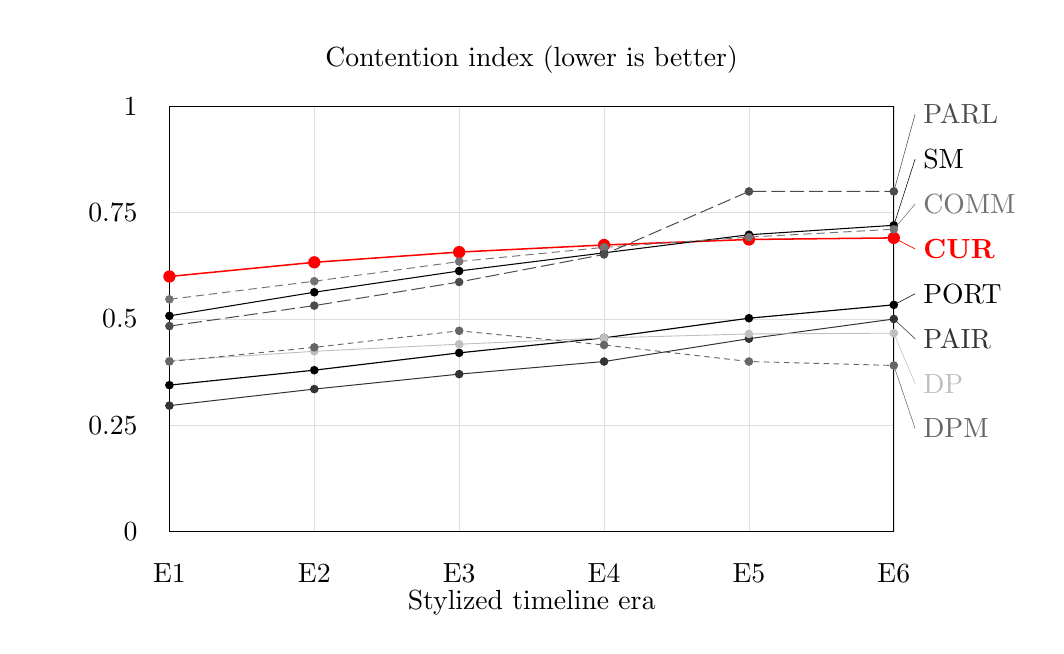
\begin{tikzpicture}[x=1mm,y=1mm]
\path[use as bounding box] (0,0) rectangle (128.0,76.0);
\draw[black!13,line width=0.18pt] (18.0,12.0) -- (110.0,12.0);
\node[anchor=east] at (15.2,12.0) {0};
\draw[black!13,line width=0.18pt] (18.0,25.5) -- (110.0,25.5);
\node[anchor=east] at (15.2,25.5) {0.25};
\draw[black!13,line width=0.18pt] (18.0,39.0) -- (110.0,39.0);
\node[anchor=east] at (15.2,39.0) {0.5};
\draw[black!13,line width=0.18pt] (18.0,52.5) -- (110.0,52.5);
\node[anchor=east] at (15.2,52.5) {0.75};
\draw[black!13,line width=0.18pt] (18.0,66.0) -- (110.0,66.0);
\node[anchor=east] at (15.2,66.0) {1};
\draw[black!12,line width=0.18pt] (18.0,12.0) -- (18.0,66.0);
\node[anchor=north] at (18.0,9.2) {E1};
\draw[black!12,line width=0.18pt] (36.4,12.0) -- (36.4,66.0);
\node[anchor=north] at (36.4,9.2) {E2};
\draw[black!12,line width=0.18pt] (54.8,12.0) -- (54.8,66.0);
\node[anchor=north] at (54.8,9.2) {E3};
\draw[black!12,line width=0.18pt] (73.2,12.0) -- (73.2,66.0);
\node[anchor=north] at (73.2,9.2) {E4};
\draw[black!12,line width=0.18pt] (91.6,12.0) -- (91.6,66.0);
\node[anchor=north] at (91.6,9.2) {E5};
\draw[black!12,line width=0.18pt] (110.0,12.0) -- (110.0,66.0);
\node[anchor=north] at (110.0,9.2) {E6};
\draw[black,line width=0.28pt] (18.0,12.0) rectangle (110.0,66.0);
\draw[red,line width=0.55pt] (18.0,44.4) -- (36.4,46.2) -- (54.8,47.5) -- (73.2,48.4) -- (91.6,49.1) -- (110.0,49.3);
\fill[red] (18.0,44.4) circle[radius=0.78];
\fill[red] (36.4,46.2) circle[radius=0.78];
\fill[red] (54.8,47.5) circle[radius=0.78];
\fill[red] (73.2,48.4) circle[radius=0.78];
\fill[red] (91.6,49.1) circle[radius=0.78];
\fill[red] (110.0,49.3) circle[radius=0.78];
\draw[black,line width=0.38pt] (18.0,39.4) -- (36.4,42.4) -- (54.8,45.1) -- (73.2,47.4) -- (91.6,49.7) -- (110.0,50.9);
\fill[black] (18.0,39.4) circle[radius=0.55];
\fill[black] (36.4,42.4) circle[radius=0.55];
\fill[black] (54.8,45.1) circle[radius=0.55];
\fill[black] (73.2,47.4) circle[radius=0.55];
\fill[black] (91.6,49.7) circle[radius=0.55];
\fill[black] (110.0,50.9) circle[radius=0.55];
\draw[black!55,line width=0.34pt,dash pattern=on 3pt off 1.8pt] (18.0,41.5) -- (36.4,43.8) -- (54.8,46.3) -- (73.2,48.1) -- (91.6,49.4) -- (110.0,50.4);
\fill[black!55] (18.0,41.5) circle[radius=0.55];
\fill[black!55] (36.4,43.8) circle[radius=0.55];
\fill[black!55] (54.8,46.3) circle[radius=0.55];
\fill[black!55] (73.2,48.1) circle[radius=0.55];
\fill[black!55] (91.6,49.4) circle[radius=0.55];
\fill[black!55] (110.0,50.4) circle[radius=0.55];
\draw[black!70,line width=0.36pt,dash pattern=on 5pt off 1.8pt] (18.0,38.1) -- (36.4,40.7) -- (54.8,43.7) -- (73.2,47.2) -- (91.6,55.2) -- (110.0,55.2);
\fill[black!70] (18.0,38.1) circle[radius=0.55];
\fill[black!70] (36.4,40.7) circle[radius=0.55];
\fill[black!70] (54.8,43.7) circle[radius=0.55];
\fill[black!70] (73.2,47.2) circle[radius=0.55];
\fill[black!70] (91.6,55.2) circle[radius=0.55];
\fill[black!70] (110.0,55.2) circle[radius=0.55];
\draw[black!80,line width=0.36pt] (18.0,28.0) -- (36.4,30.1) -- (54.8,32.0) -- (73.2,33.6) -- (91.6,36.5) -- (110.0,39.0);
\fill[black!80] (18.0,28.0) circle[radius=0.55];
\fill[black!80] (36.4,30.1) circle[radius=0.55];
\fill[black!80] (54.8,32.0) circle[radius=0.55];
\fill[black!80] (73.2,33.6) circle[radius=0.55];
\fill[black!80] (91.6,36.5) circle[radius=0.55];
\fill[black!80] (110.0,39.0) circle[radius=0.55];
\draw[black,line width=0.42pt] (18.0,30.6) -- (36.4,32.5) -- (54.8,34.7) -- (73.2,36.6) -- (91.6,39.1) -- (110.0,40.8);
\fill[black] (18.0,30.6) circle[radius=0.55];
\fill[black] (36.4,32.5) circle[radius=0.55];
\fill[black] (54.8,34.7) circle[radius=0.55];
\fill[black] (73.2,36.6) circle[radius=0.55];
\fill[black] (91.6,39.1) circle[radius=0.55];
\fill[black] (110.0,40.8) circle[radius=0.55];
\draw[black!25,line width=0.32pt] (18.0,33.7) -- (36.4,34.9) -- (54.8,35.8) -- (73.2,36.6) -- (91.6,37.1) -- (110.0,37.2);
\fill[black!25] (18.0,33.7) circle[radius=0.55];
\fill[black!25] (36.4,34.9) circle[radius=0.55];
\fill[black!25] (54.8,35.8) circle[radius=0.55];
\fill[black!25] (73.2,36.6) circle[radius=0.55];
\fill[black!25] (91.6,37.1) circle[radius=0.55];
\fill[black!25] (110.0,37.2) circle[radius=0.55];
\draw[black!60,line width=0.34pt,dash pattern=on 2pt off 1.6pt] (18.0,33.6) -- (36.4,35.4) -- (54.8,37.5) -- (73.2,35.7) -- (91.6,33.6) -- (110.0,33.1);
\fill[black!60] (18.0,33.6) circle[radius=0.55];
\fill[black!60] (36.4,35.4) circle[radius=0.55];
\fill[black!60] (54.8,37.5) circle[radius=0.55];
\fill[black!60] (73.2,35.7) circle[radius=0.55];
\fill[black!60] (91.6,33.6) circle[radius=0.55];
\fill[black!60] (110.0,33.1) circle[radius=0.55];
\draw[black!60,line width=0.2pt] (110.0,33.1) -- (112.7,25.1);
% legend-label label=DPM x=113.5 y=25.1
\node[anchor=west,inner sep=0.5pt,text=black!60] at (113.5,25.1) {DPM};
\draw[black!25,line width=0.2pt] (110.0,37.2) -- (112.7,30.8);
% legend-label label=DP x=113.5 y=30.8
\node[anchor=west,inner sep=0.5pt,text=black!25] at (113.5,30.8) {DP};
\draw[black!80,line width=0.2pt] (110.0,39.0) -- (112.7,36.5);
% legend-label label=PAIR x=113.5 y=36.5
\node[anchor=west,inner sep=0.5pt,text=black!80] at (113.5,36.5) {PAIR};
\draw[black,line width=0.2pt] (110.0,40.8) -- (112.7,42.2);
% legend-label label=PORT x=113.5 y=42.2
\node[anchor=west,inner sep=0.5pt,text=black] at (113.5,42.2) {PORT};
\draw[red,line width=0.25pt] (110.0,49.3) -- (112.7,47.9);
% legend-label label=CUR x=113.5 y=47.9
\node[anchor=west,inner sep=0.5pt,text=red] at (113.5,47.9) {\textbf{CUR}};
\draw[black!55,line width=0.2pt] (110.0,50.4) -- (112.7,53.6);
% legend-label label=COMM x=113.5 y=53.6
\node[anchor=west,inner sep=0.5pt,text=black!55] at (113.5,53.6) {COMM};
\draw[black,line width=0.2pt] (110.0,50.9) -- (112.7,59.3);
% legend-label label=SM x=113.5 y=59.3
\node[anchor=west,inner sep=0.5pt,text=black] at (113.5,59.3) {SM};
\draw[black!70,line width=0.2pt] (110.0,55.2) -- (112.7,65.0);
% legend-label label=PARL x=113.5 y=65.0
\node[anchor=west,inner sep=0.5pt,text=black!70] at (113.5,65.0) {PARL};
\node at (64.0,3.0) {Stylized timeline era};
\node[anchor=south] at (64.0,69.0) {Contention index (lower is better)};
\end{tikzpicture}
\endgroup

  \caption{Rising-contention stress path from the main comparison campaign. The index combines gridlock, compromise loss, and weak public-mandate passage. Lower is better. This is a parameterized stress path, not an endogenous causal model of polarization.}
  \label{fig:timeline-contention}
  \Description{Line chart of contention over six stylized eras.}
\end{figure}

Three patterns are observed. First, thresholds alone are weak design language: supermajority and conventional baselines suppress weak mandates by suppressing throughput, while open default enactment reverses the problem. Second, agenda and content mechanisms matter across families: alternatives, amendment tournaments, petitions, open calendars, discharge, citizen review, initiatives, objection windows, and harm rules change who can force attention and at what cost. Third, reversibility is separate: judicial and law-registry review reduce exposure to weak or rights-risky laws but can increase volatility.

The exploratory result does not support a single dominant rule. The portfolio hybrid turns the pattern into a testable design: fast lanes for low-risk proposals, stronger consent or revision for risky proposals, proposer accountability, influence disclosure, alternatives before binary ratification, affected-group protection, and review of uncertain laws. Its mixed result is useful: combining good mechanisms improves several risk diagnostics, but adds administrative load and does not dominate simpler pairwise alternatives.

\section{Limitations}

The model is stylized. It uses one primary policy dimension, generated legislators, generated support and benefit, simplified issue domains, and abstract lobbying units. Public-mandate diagnostics distinguish salience and costly affected-group pressure from cheap amplified volume, but they are still proxies. Because public benefit is internal to the generator, welfare comparisons are conditional on model assumptions. Systems that screen extreme, uncertain, or lobby-heavy bills may look better partly because the generator often encodes those features as lower expected public value. Adversarial cases partially relax this assumption, but welfare remains a synthetic signal, not an empirical social-welfare estimate.

The calibration layer screens conventional baselines against empirical ranges, and the empirical bridge currently covers six raw validation inputs. That is enough to make several agenda-access and representation proxies inspectable, but it is not enough for model validation or parameter fitting. The committee and sponsor summaries are derived from sampled Congress.gov bill actions and are especially rough; fixture samples exercise adapter shapes but are not validation data. Strategic behavior remains bounded: proposers and lobby groups adapt, and norm erosion can raise delay, but parties, committees, coalitions, courts, agencies, media, and elections do not yet co-evolve. Chamber scenarios are sensitivity prototypes. Citizen panels, initiatives, objection windows, tournaments, audits, challenge tokens, judicial review, and law-registry review are optimistic prototypes whose costs are represented only indirectly. Package bargaining models side payments, delay, jurisdictional trades, and distributive load, not legal text or appropriations.

\section{Reproducibility}

The submitted manuscript is anonymized for double-blind review. The reproducibility package contains source code, generated reports, the ODD+D appendix, and scripts. \texttt{make paper-checks} regenerates the campaign, diagnostics, figures, PDFs, word-count check, anonymity scan, figure-label and table consistency checks, and PDF manifest. \texttt{make supplement-anonymous} builds the double-blind supplement. Optional fixture samples can be refreshed with \texttt{make fetch-validation-samples}; they remain separate from raw validation inputs. \texttt{make build-bill-progression-raw} rebuilds the Congress.gov bill-progression sample, and \texttt{make build-core-raw-validation} rebuilds the broader Voteview, Congress.gov-derived, and LDA bridge samples when network access and any required API key are available.

\section*{Use of Large Language Model Tools}

The research question and core simulator idea originated with the human author. Large language model tools were used for software implementation assistance and for drafting, editing, and reorganizing manuscript text. The author reviewed and is responsible for all code, experiments, reported results, text, and citations. No large language model is listed as an author.

\section{Conclusion}

This paper argues for computational mechanism search as a way to study legislative design. Default enactment is one stress case, but the broader contribution is comparing ordinary and unusual institutional bundles under common assumptions. The prototype suggests that compromise and productivity depend on combinations of agenda access, contestation, mediation, alternative selection, anti-capture safeguards, affected-group protection, and reversibility rather than any single passage threshold. The portfolio hybrids are synthesized candidates; the next step is to fit and stress-test their public-opinion, influence-system, court-review, and bargaining submodels rather than treating either as final.

\bibliographystyle{ACM-Reference-Format}
\bibliography{references}

\end{document}
